\documentclass[11pt]{jarticle}
\usepackage[dvipdfmx]{graphicx}
\usepackage{kcctd-report}
\usepackage{booktabs}
\usepackage{mathcomp}
\usepackage{array}
\usepackage{mathtools,amssymb}
\usepackage{siunitx}
\usepackage{multirow}
\usepackage{tabularx}
\usepackage{subcaption}
\usepackage{float}
\usepackage{listings,jvlisting}
\lstset{
	basicstyle={\ttfamily},
	identifierstyle={\small},
	commentstyle={\smallitshape},
	keywordstyle={\small\bfseries},
	ndkeywordstyle={\small},
	stringstyle={\small\ttfamily},
	frame={tb},
	breaklines=true,
	columns=[l]{fullflexible},
	numbers=left,
	xrightmargin=0zw,
	xleftmargin=3zw,
	numberstyle={\scriptsize},
	stepnumber=1,
	numbersep=1zw,
	lineskip=-0.5ex,
	tabsize=2
}
\renewcommand{\lstlistingname}{ソースコード}

\title{MOS構造の作製と特性評価}
\adviser{西 敬生 教授}

\sdate{令和5年6月15日}
\edate{令和5年6月22日}
\fdate{令和5年6月27日}
\rdate{}

\grade{5}
\anumber{12}
\gnumber{B}
\name{河合 将暉}
\jname{}
\comment{}
\begin{document}
\maketitle

\section{目的}
	トランジスタ製作の基本技術の習得とMOSトランジスタの基本特性であるMOS容量の電圧依存性,周波数特性および酸化膜厚の参加時間依存性について学ぶ.

\section{解説}
	\subsection{MOS構造}
		MOSとはMetal(金属)−Oxied(酸化膜)−Semiconductor(半導体)の頭文字の略称である.
		半導体Siの表面を酸化させ,絶縁体酸化膜\,$\mathrm{SiO_{2}}$が形成される.
		この上に金属電極を積むことで図\refeq{}のMOS構造が形成される.

	\subsection{作製過程}
		\begin{enumerate}
			\item ウェーハ洗浄\\
				Siウェーハの表面は一度パッケージから出してしまえば,たとえクリーンルーム内といえども,多かれ少なかれ汚染される.
				本校クリーンルームはクラス10000(1立方フィート内に$0.5\,\mu$\,mの粒子が1万粒)とされ,専門家ではない学生が扱うことを考えれば,ウェーハを扱う企業の現場(クラス1〜100)より非常に汚染されやすい環境にある.
				具体的にウェーハ表面を汚染するものや除去したいものとしては

				\begin{enumerate}
					\item パーティクル\\
					\item アルカリ金属,重金属\\
					\item 有機物\\
					\item Si自然酸化膜\\
				\end{enumerate}

				以上が挙げられる.
				ここでのパーティクルとは,材質などは問わずに,粒形が数百nm以上のものの総称である.

				これらをウェーハ表面に物理的・科学敵にダメージを与えることなく,除去する洗浄方法が必要とされており,RCA法など,多くの方法が提案されている.

			\item 酸化膜形成\\
				Siの酸化膜はウェーハを,酸素を満たした$900〜1200^\circ$ の高温の炉中に入れr熱酸化によって形成されることが多い.
				満たす酸素の供給源としては,乾燥した純粋な酸素$\mathrm{O_{2}}$を送り込むドライ酸化と,水蒸気または水素と酸素の混合気を送り込むウェット(水蒸気またはスチームなどともいう)酸化がある.

				酸化のメカニズムは,

				\begin{enumerate}
					\item 酸化種($\mathrm{O_{2}}$または$\mathrm{H_{2}O}$)が表面で反応もしくは$\mathrm{SiO_{2}}$に吸着される.\\
					\item 吸着された$\mathrm{O}_{2}$または$\mathrm{H_{2}O}$が酸化膜$\mathrm{SiO_{2}}$の中を拡散してシリコンの界面に達する.\\
					\item シリコンとの界面でシリコンと反応して$\mathrm{SiO_{2}}$になる.\\
				\end{enumerate}
				
				といった段階を経る.
				酸化速度は酸化膜$\mathrm{SiO_{2}}$が薄い時には3の化学反応の速度で決まり,厚い時には2の拡散する速度によって決まる.
				前者の状況を反応律速,後者を供給律速という.

				全体の反応を式で表すと
				\begin{equation}
					T^{2}_{OX} + AT_{OX} = B(t+\tau_{0})
				\end{equation}

				となり,ここでA,Bは温度と酸化条件で決まる定数,$\tau_{0}$は初期の酸化膜厚に対応する定数である.
				酸化時間tが長くて,$T_{OX}$が厚いときには

				\begin{equation}
					T_{OX}^{2}\backsimeq (B/A)(t+\tau_{0})
				\end{equation}

				となる.
				これらの酸化定数を表\refeq{tab:Sidrai}に示す.

				\begin{table}[H]
				\begin{center}
				\caption{シリコンのドライ酸化時の酸化定数}
				\label{tab:Sidrai}
				\begin{tabular}{cSSS} \toprule
					酸化温度T\,[$^\circ \mathrm{C}$]&A[$\mathrm{\mu m}$]&B[$\mathrm{\mu m^{2}/h}$]&$\tau_{0}$[h]\\ \hline
					1200&0.040&0.045&0.027\\
					1100&0.090&0.027&0.076\\
					1000&0.165&0.0117&0.37\\
					920&0.235&0.0049&1.40\\
					800&0.370&0.0011&9.0\\ \bottomrule
				\end{tabular}
				\end{center}
				\end{table}

			\item フォトリソグラフィ
				IC製造において各種材料膜を所望の形状加工にするため,パターニングを施すことをフォトリソグラフィと呼ぶ.
				この工程は通常の写真技術の応用であり,以下の手順を踏む.
				\begin{enumerate}
					\item レジスト塗布(感光剤塗布):ウェーハ上にフォトレジストという感光性樹脂をコーティング
					\item 露光:平面的パターンが書かれたマスクを通し,光を照射して,パターンをレジストに転写
					\item レジスト部分除去:レジストの化学反応により変質した部分を除去することでマスクパターンと同じレジストパターンが形成される.
					\item 加工:部分的なレジストの除去により,レジストの下の層が一部分,表出.その表出部分をエッチングしたり,上から蒸着や塗布などを行ったりすることで,パターンと同じ構造を形成できる.
				\end{enumerate}

				$\boldsymbol{レジスト}$\\
					レジストには光が当たった部分が残るネガ型と,光が当たった部分が解けて取れるポジ型があり,本実験ではポジ型のOFPRという商品名で,光が当たるとアルカリ溶液に可溶性となる.
					レジストの塗布にはスピナー(スピンコーター)と呼ばれる塗布機を用いる.
					これはウェーハにレジストを滴下後高速回転させることで一定の膜厚のレジストのコーティングを可能とする.\\
				\\
				$\boldsymbol{露光}$\\
					マスク粗いなと呼ばれる.マスク接触型の露光装置で行われる.光学ステージへのセットは自動で行われる.
					露光の高原には高圧水銀ランプから発せられる紫外線(i線,波長$\lambda = 365$nm)


			\item フォトリソグラフィ\\
				IC製造において各材料膜を所望の形状に加工するため,パターニングを施すことをフォトリソグラフィと呼ぶ.
				この工程は通常の写真技術の応用であり,以下の手順を踏む.
				\begin{enumerate}
					\item レジスト塗布(感光剤塗布)\\
						ウェーハ上にフォトレジストという感光性樹脂をコーティング
					\item 露光\\
						平均的パターンが描かれたマスクを通し,光を照射して,パターンをレジストに転写
					\item レジスト部分除去\\
						レジストの光化学反応により変質した部分を除去することで,マスクパターンと同じレジストパターンが形成される.
					\item 加工\\
						部分的なレジストの除去により,レジストの下の層が一部分表出する.
						その表出部分をエッチングしたり,上から蒸着や塗布を行うことで,パターンと同じ構造を形成できる.
				\end{enumerate}
		\end{enumerate}

	\subsection{MOS構造の電気的特性}
		\begin{enumerate}
			\item 電圧印加による3つの状態\\
				MOS構造は,図\refeq{}のように印加電圧によって電気的に3つの状態に変化する.
				図\refeq{}はプラスの電圧V1を印加した状態で,酸化膜を挟んで電極下の半導体の部分に電子が引き寄せられ,多数キャリアの正孔と引き寄せられた電子が再結合し,キャリアの存在しない空乏層と呼ばれる領域が生じる.
				これを空乏状態という.
				V1より大きな電圧を印加するとより多く電子が引き寄せられ,酸化膜−半導体界面のごく薄い部分だけP形からN形に``反転''する.
				これを図\refeq{}のように反転層といい,反転状態と呼ぶ.
				このようにMOS構造では,半導体の伝導型を電圧によって変化させることができる.
				MOSトランジスタはこれを利用している.
				図\refeq{}は蓄積状態と呼ばれ,V3を印加すると正孔を引き寄せ,その部分の抵抗率が下げられる.

			\item 電圧−容量特性\\
				MOS構造は金属で絶縁体をサンドイッチしていると考えるとコンデンサの一種と見ることもできる.
				空乏層という絶縁層を生じさせ,印加電圧によって空乏層幅を変化させられるため,静電容量も変えることができる.
				図\refeq{}はMOS構造のC−V特性で周波数によって特性が図のように変化する.

		\end{enumerate}

\section{実験方法}
	\subsection{使用器具}
		本実験での使用器具を表\refeq{tab:used}に示す.
		\begin{table}[H]
		\begin{center}
		\caption{使用器具}
		\label{tab:used}
		\begin{tabular}{clllll} \toprule
		No&\multicolumn{1}{l}{機器名}&\multicolumn{1}{l}{型番}&\multicolumn{1}{l}{シリアルNo}&\multicolumn{1}{l}{備考}\\ \hline
		1&横型管状電気炉&&&\\
		2&ドラフター&&&\\
		3&スピンコーター&&&\\
		4&ジェットオーブン&&&\\
		5&真空蒸着装置&&&\\
		6&超音波洗浄機&&&\\
		7&ホットプレート&&&\\
		8&マスクアライナ&&&\\
		9&顕微鏡&&&\\
		10&LCRメータ&&&\\
		11&定電圧電源&&&\\
		12&グローブボックス&&&\\
		13&シリコン基板&&&\\ \bottomrule
		\end{tabular}
		\end{center}
		\end{table}

	\subsection{実験方法}
		MOS構造の作成工程を図\refeq{}に示す.
		図\refeq{}で完成したMOS構造の静電容量−電圧特性,周波数依存性を測定した.
		作成手順を以下に示す.
		\begin{enumerate}
			\item プライムウェーハ初期洗浄\\
				排気装置であるドラフターの中で表\refeq{tab:wash}の手順に従って洗浄作業を行った.
				\begin{table}[H]
				\begin{center}
				\caption{初期洗浄方法}
				\label{tab:wash}
				\begin{tabular}{c|ccc} \toprule
					手順&洗浄方法&時間\,[分]&使用ビーカ\\ \hline
					1&セミコクリーン23による超音波洗浄&5&セミコクリーン\\
					2&純水オーバーフロー&5&セミコクリーン−$\mathrm{H_{2}O}$\\
					3&遠心乾燥&1&\\ \bottomrule
				\end{tabular}
				\end{center}
				\end{table}

			\item 酸化膜形成\\
				酸化膜形成の条件を以下に示す.
				\begin{itemize}
					\item 電気炉の温度:$1060^\circ \mathrm{C}$
					\item レギュレータ圧力:酸素 3\,L/min,窒素 3\,L/min
					\item ガス流量:酸素 1\,kg/$\mathrm{cm^{2}}$,窒素 1.2\,kg/$\mathrm{cm^{2}}$
					\item 酸化時間:50分,65分,80分
				\end{itemize}
				実際には電気炉を稼働させてから最初の20分は温度が安定せず,一時的に$1160^\circ \mathrm{C}$まで上昇した.

				次に,酸化膜形成の手順を以下に示す.
				\begin{enumerate}
					\item 窒素を流すスイッチ(1−SV)がONで,窒素フローメーターが3\,L/minであることを確認した.
					\item ウェーハを石英製ホルダーにセットし,そのホルダーごと電気炉の入口の手前(電気炉の外)に置いた.
					\item 手袋をし,電気炉の入口に石英棒で,ウェーハをゆっくりと中央に挿入し,蓋をした.
					\item 酸素を流すスイッチ(2‐SV)をON,酸素フローメータが3\,L/minであることを確認した.
					\item 1−SVをOFF,窒素を0にした.
					\item 酸化時間後,1−SVをON,窒素フローメータ3\,L/minであることを確認した.
					\item 2−SVをOFF,酸素を0にした.
					\item 手袋をし,電気炉の蓋を取った.
					\item ウェーハをゆっくりと取り出し,入口のところで2分間置いた.
					\item 電気炉の外まで引出し,3分置いた後,トレイからウェーハを1枚取った.
					\item (c)に戻り,全てのウェーハを所定時間酸化し終わるまで続けた.
				\end{enumerate}

			\item 表面Al蒸着\\
				ゲートとなる金属(Al)をウェーハ表面に蒸着した.
				蒸着減となるタングステンヒータとAl塊を表\refeq{tab:tangsten}のように有機洗浄した.
				その後,真空蒸着装置にウェーハ,タングステンヒータとAl塊をセットし,装置内を真空にした後,蒸着.
				\begin{table}[H]
				\begin{center}
				\caption{タングステンヒータとアルミの有機洗浄方法}
				\label{tab:tangsten}
				\begin{tabular}{c|ccc} \toprule
					手順&洗浄方法&時間\,[分]&使用ビーカ\\ \hline
					1&アセトン&5&AL‐US\\
					2&メタノール&5&AL‐US\\
					3&アセトン&5&AL‐US\\
					4&メタノール&5&AL‐US\\
					5&ホットプレート上で乾燥&&\\ \bottomrule
				\end{tabular}
				\end{center}
				\end{table}
			\item フォトリソグラフィ\\
				蒸着したAl薄膜を2mm角の電極パターンとして形成するため,フォトリソグラフィを行った.
				使ったレジストは感光部が溶けるポジ型を使用するため,定着液も必要となった.
				窒素中プリべークのあと,コンタクトアライナ方式により露光され,現像後,ポストベークを行った.
				フォトリソグラフィの手順は以下に示す.
				\begin{enumerate}
					\item ジェットオーブンの設定温度が110度,窒素流量が5\,L/minであることを確認した.
					\item ウェーハを金属網の上に載せ,網ごとジェットオーブンに入れ,3分間ベーキングを行った.
					\item ジェットオーブンから網ごとウェーハを取り出した.
					\item スピナーの電源が入っていること,壁にある真空弁が開いていることを確認した.
					\item スピナーの中央部にある試料台にAl電極面を上に向けてウェーハを置いた.
					\item 真空チャックスイッチをONにした.
					\item 定着液(OAP)をスポイトで滴下後,スピナーをスタートさせた.
					\item ポジレジスト(OFPR‐800)をスポイトで滴下した.レジストの粘度が高いため,直径2.5cm程度の円になるように多めに滴下する.
					\item ウェーハを網の上に置き,残りのウェーハも同様の手順を行った.
					\item ジェットオーブンに網ごとウェーハを入れ,90秒ベーキングを行った.
					\item 網ごとウェーハをマスクアライナのところに運んだ.
					\item マスクアライナのマスクホルダ両脇にあるマスクロックレバーを外側に向け,リリースした.
					\item マスクフォルダを持ち上げて開き,試料台の中心が合い,円の中に試料が入るようにウェーハを設置した.
					\item 試料固定ボタンをONにした.
					\item マスクフォルダを閉じ,両脇のマスクロックレバーを内側にしてロックした.
					\item マスクパターンがウェーハのAlの中に完全に収まるようにX,Yまわしで調整した.
					\item 試料台Z軸動作ボタンをONにして,8秒間露光した.
					\item ランプハウスを後ろに移動させ,試料台Z軸動作ボタンをOFFにした.
					\item マスクホルダの両脇のマスクロックレバーを外側にして,リリースし,マスクホルダを開いた.
					\item 試料固定スイッチをOFFにし,試料を取り出した.残りのウェーハについても同様に行った.
					\item 露光を終えたウェーハをフッ素樹脂製ディッパーに装着した.
					\item 2台のスターラーの電源が入っていることを確認した.
					\item ウェーハを1枚ずつ,撹拌中の現像液の中に2分間ディッパーごと浸した.感光した部分だけのレジストが落ち,マスクの模様が反転出現することを確認した.
					\item ウェーハ上の水分を飛ばすため,窒素ガンでウェーハに対して窒素を吹きかけた.
					\item 窒素流量5\,L/minのジェットオーブンにウェーハを入れ,$110\,^\circ \mathrm{C}$ で3分間ベーキングを行った.
				\end{enumerate}

			\item Alエッチング\\
				パターン通りにAlエッチングし,電極を形成する.
				エッチングの条件は表\refeq{tab:aletching}に示す.
				\begin{table}[H]
				\begin{center}
				\caption{アルミエッチングの方法}
				\label{tab:aletching}
				\begin{tabular}{c|cccc} \toprule
					手順&洗浄方法&温度\,[$^\circ \mathrm{C}$]&時間\,[分]&使用ビーカ\\ \hline
					1&エッチング液 泡が出なくなるまで浸す&43&泡が出なくなるまで&AL‐ETCH\\
					2&純水オーバーフロー&&1&AL‐$\mathrm{H_{2}O}$\\
					3&遠心乾燥&&1&\\ \bottomrule
				\end{tabular}
				\end{center}
				\end{table}
				エッチング液はホットプレートで43度に上げた.
				温度はエッチング液に入れた温度計で測定した.
				43度のエッチング液は高い粘性を示した.
				ウェーハを単独で入れてしまうと後で取り出しにくいので,ウェーハはピンセットに挟んだまま液に浸した.
				Alの溶液はエッチング液中に気泡が生じることによって確認できた.
				泡がなくなったとき,エッチングを終了し,純水オーバーフローを行った.

			\item レジスト除去\\
				Al電極上のレジストを有機溶媒で除去.
				ウェーアトレーごと洗浄し,メタノールに浸すときはホットプレートを使用した.
				表\refeq{tab:resistwash}にレジスト除去の方法を示す.
				\begin{table}[H]
				\begin{center}
				\caption{レジスト除去の方法}
				\label{tab:resistwash}
				\begin{tabular}{c|cccc} \toprule
					手順&洗浄方法&温度\,[$^\circ \mathrm{C}$]&時間\,[分]&使用ビーカ\\ \hline
					1&リンス1&&3&AL‐RINSE1\\
					2&リンス2&&1&AL‐RINSE1\\
					3&アセトン&&浸す&AL‐ACETONE\\
					4&メタノール&沸騰&浸す&AL‐METHANOL\\
					5&ホットプレートの紙上で乾燥&150&&\\ \bottomrule
				\end{tabular}
				\end{center}
				\end{table}

			\item 表面レジスト塗布\\
				この後の行程の裏面酸化膜エッチングでの表面酸化膜および,Al電極の保護のため,表面をレジストでコーティングした.
				手順はフォトリソグラフィの(a)から(j)までをもう一度行った.

			\item 裏面酸化膜エッチング\\
				エッチングにはバッファードフッ酸を用いた.
				シリコンはバッファードフッ酸に対して撥水性を有するためウェーハがエッチング液をはじくのを確認したら,その後30秒間フッ酸に浸し,純水オーバーフローを行った.
				以下に手順を表\refeq{tab:uraetching}に示す.
				\begin{table}[H]
				\begin{center}
				\caption{裏面酸化膜エッチングの方法}
				\label{tab:uraetching}
				\begin{tabular}{c|ccc} \toprule
					手順&洗浄方法&時間\,[分]&使用ビーカ\\ \hline
					1&バッファードフッ酸&ウェーハがフッ酸をはじくまで +0.5&G‐BHF\\
					2&純水オーバーフロー&5&G‐$\mathrm{H_{2}O}‐BHF$\\
					3&遠心乾燥&1&\\ \bottomrule
				\end{tabular}
				\end{center}
				\end{table}

			\item レジスト除去\\
				表\refeq{tab:resistwash}と同様の手順で表面のレジストを除去した.

			\item Al蒸着\\
				タングステンヒータとアルミ塊の洗浄を行い表面と同様にアルミ蒸着を行った.
				ウェーハは裏面酸化膜エッチングしたものを蒸着装置にセットした.
		\end{enumerate}

		\subsection{測定方法}
			\begin{enumerate}
				\item アルミゲート電極面積測定\\
					\begin{enumerate}
						\item 測定前に標準器により,較正を行った.
						\item アルミ電極の大きさは2mm角や4mm角とされているが,今回は2mm角のアルミ電極に対して顕微鏡を用いて正確な電極面積を測定した.
						\item 実験時間の都合上,班員1名が測定したデータをそのまま測定値として結果に用いた.
					\end{enumerate}
				\item 容量測定\\
					\begin{enumerate}
						\item グローブボックス内のプローブにウェーハをセットした.
						\item 定電圧電源により,酸化膜上のアルミ電極(ゲート)に外部電圧を加えた.\\印加電圧は±10Vの範囲で容量が大きく変化する間隔で測定を行った.
						\item 電圧印加時の静電容量をLCRメータを用いて測定した.
						\item 測定周波数1k, 10k,100k, 1Mの4種類を測定した.
					\end{enumerate}
			\end{enumerate}

	\section{実験結果}
		\subsection{アルミゲート電極面積測定}
			
		\subsection{容量測定}
			\begin{table}[H]
			\begin{center}
			\caption{酸化時間50分のウェーハの電圧‐容量特性}
			\label{tab:wehacap50}
			\begin{tabular}{S|SSSS} \toprule
				&\multicolumn{4}{c}{周波数\,[kHz]ごとの静電容量\,[nF]}\\ \hline
				印加電圧\,[V]&\multicolumn{1}{c}{1000}&\multicolumn{1}{c}{100}&\multicolumn{1}{c}{10}&\multicolumn{1}{c}{1}\\ \hline
				-10 & 1.51 & 1.45 & 1.44 & 1.44 \\
				-8 & 1.51 & 1.44 & 1.44 & 1.44 \\
				-6 & 1.5 & 1.43 & 1.43 & 1.43 \\
				-4 & 1.48 & 1.41 & 1.41 & 1.41 \\
				-3 & 1.44 & 1.39 & 1.38 & 1.38 \\
				-2.8 & 1.43 & 1.37 & 1.37 & 1.37 \\
				-2.6 & 1.41 & 1.35 & 1.35 & 1.35 \\
				-2.4 & 1.38 & 1.32 & 1.32 & 1.32 \\
				-2.2 & 1.33 & 1.28 & 1.28 & 1.28 \\
				-2 & 1.25 & 1.21 & 1.21 & 1.21 \\
				-1.8 & 1.11 & 1.09 & 1.1 & 1.1 \\
				-1.6 & 0.862 & 0.911 & 0.97 & 0.946 \\
				-1.4 & 0.639 & 0.66 & 0.754 & 0.718 \\
				-1.2 & 0.524 & 0.511 & 0.535 & 0.518 \\
				-1 & 0.457 & 0.444 & 0.499 & 0.453 \\
				0 & 0.35 & 0.344 & 0.345 & 0.68 \\
				1 & 0.35 & 0.343 & 0.344 & 0.71 \\
				2 & 0.35 & 0.343 & 0.344 & 0.694 \\
				4 & 0.35 & 0.343 & 0.344 & 0.737 \\
				6 & 0.351 & 0.343 & 0.344 & 0.75 \\
				8 & 0.351 & 0.344 & 0.345 & 0.762 \\
				10 & 0.351 & 0.344 & 0.345 & 0.774 \\ 
				\bottomrule
			\end{tabular}
			\end{center}
			\end{table}

			\begin{figure}[H]
			\centering
			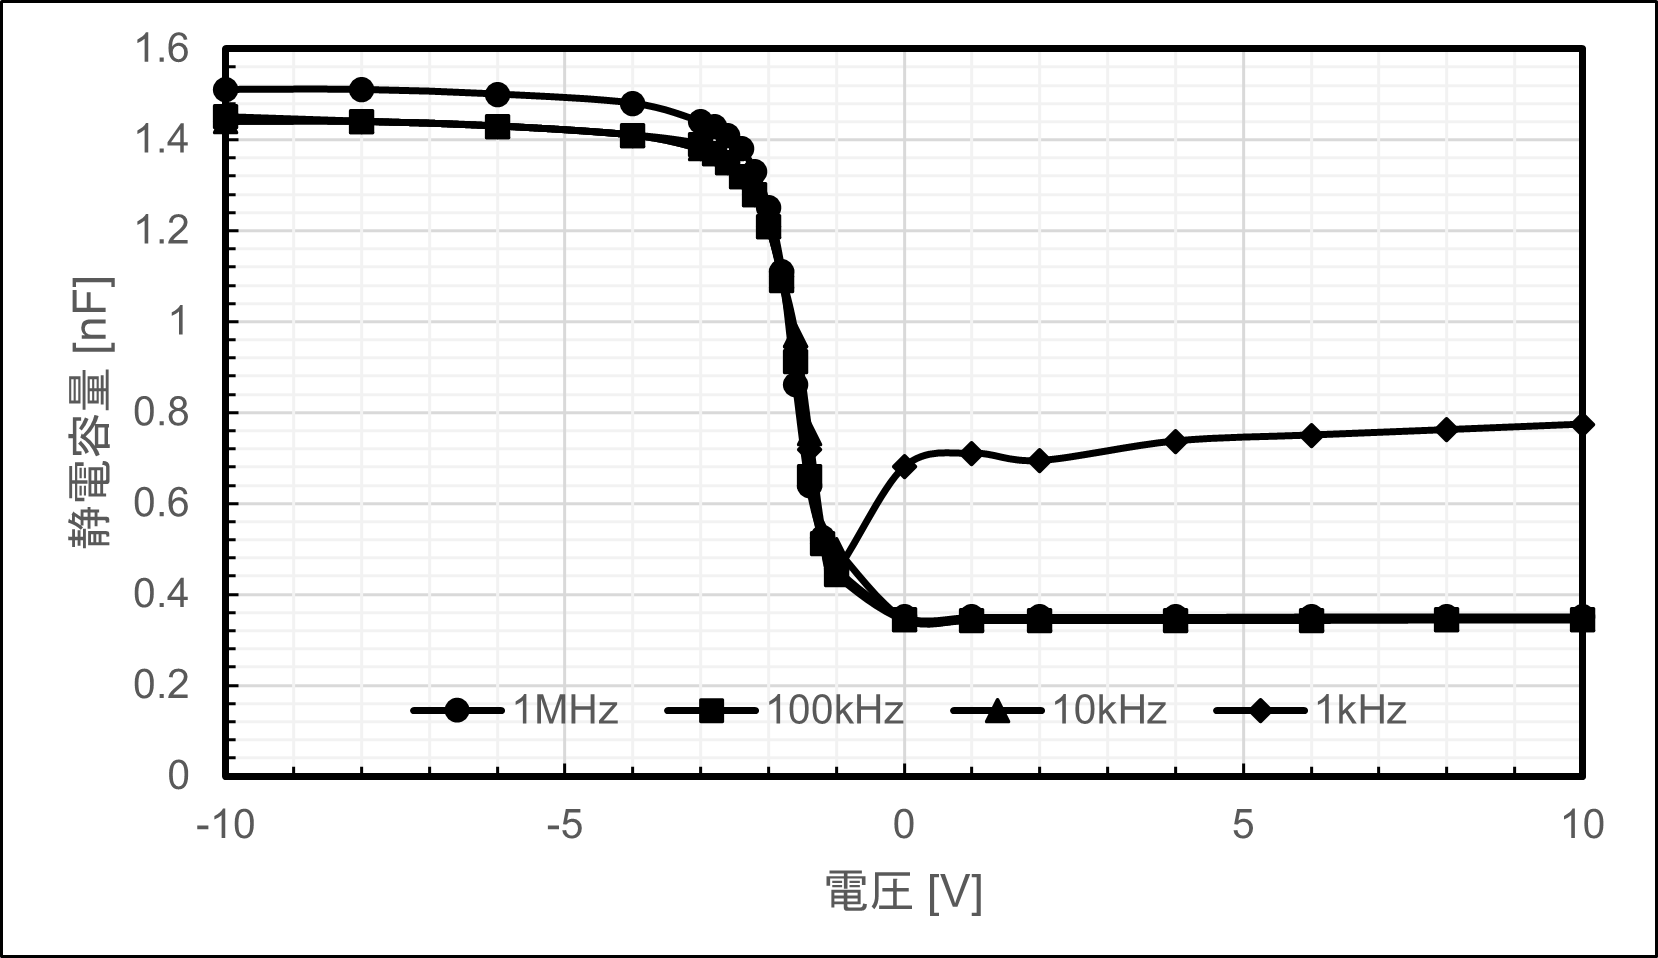
\includegraphics[width = 12cm]{figs/wehacap50.png}
			\caption{酸化時間50分のウェーハの電圧‐静電容量特性のグラフ}
			\label{fig:wehacap50}
			\end{figure}

			\begin{table}[H]
			\begin{center}
			\caption{酸化時間65分のウェーハの電圧‐容量特性}
			\label{tab:wehacap65}
			\begin{tabular}{S|SSSS} 
				\toprule
				&\multicolumn{4}{c}{周波数\,[kHz]ごとの静電容量\,[nF]}\\ \hline
				印加電圧\,[V]&\multicolumn{1}{c}{1000}&\multicolumn{1}{c}{100}&\multicolumn{1}{c}{10}&\multicolumn{1}{c}{1}\\ \hline
				-10 & 1.26 & 1.21 & 1.2 & 1.2 \\
				-8 & 1.26 & 1.2 & 1.2 & 1.2 \\
				-6 & 1.25 & 1.19 & 1.19 & 1.19 \\
				-4 & 1.23 & 1.17 & 1.18 & 1.18 \\
				-3 & 1.2 & 1.14 & 1.14 & 1.14 \\
				-2.8 & 1.18 & 1.13 & 1.13 & 1.13 \\
				-2.6 & 1.16 & 1.11 & 1.11 & 1.11 \\
				-2.4 & 1.12 & 1.08 & 1.08 & 1.08 \\
				-2.2 & 1.06 & 1.03 & 1.03 & 1.03 \\
				-2 & 0.967 & 0.962 & 0.969 & 0.97 \\
				-1.8 & 0.815 & 0.856 & 0.89 & 0.898 \\
				-1.6 & 0.634 & 0.68 & 0.767 & 0.817 \\
				-1.4 & 0.522 & 0.523 & 0.577 & 0.67 \\
				-1.2 & 0.458 & 0.448 & 0.459 & 0.537 \\
				-1 & 0.415 & 0.405 & 0.409 & 0.625 \\
				0 & 0.378 & 0.371 & 0.374 & 0.97 \\
				1 & 0.379 & 0.375 & 0.375 & 1 \\
				2 & 0.381 & 0.382 & 0.38 & 1.02 \\
				4 & 0.383 & 0.383 & 0.388 & 1.03 \\
				6 & 0.384 & 0.384 & 0.394 & 1.04 \\
				8 & 0.388 & 0.386 & 0.396 & 1.05 \\
				10 & 0.389 & 0.387 & 0.399 & 1.05 \\ 
				\bottomrule
			\end{tabular}
			\end{center}
			\end{table}

			\begin{figure}[H]
			\centering
			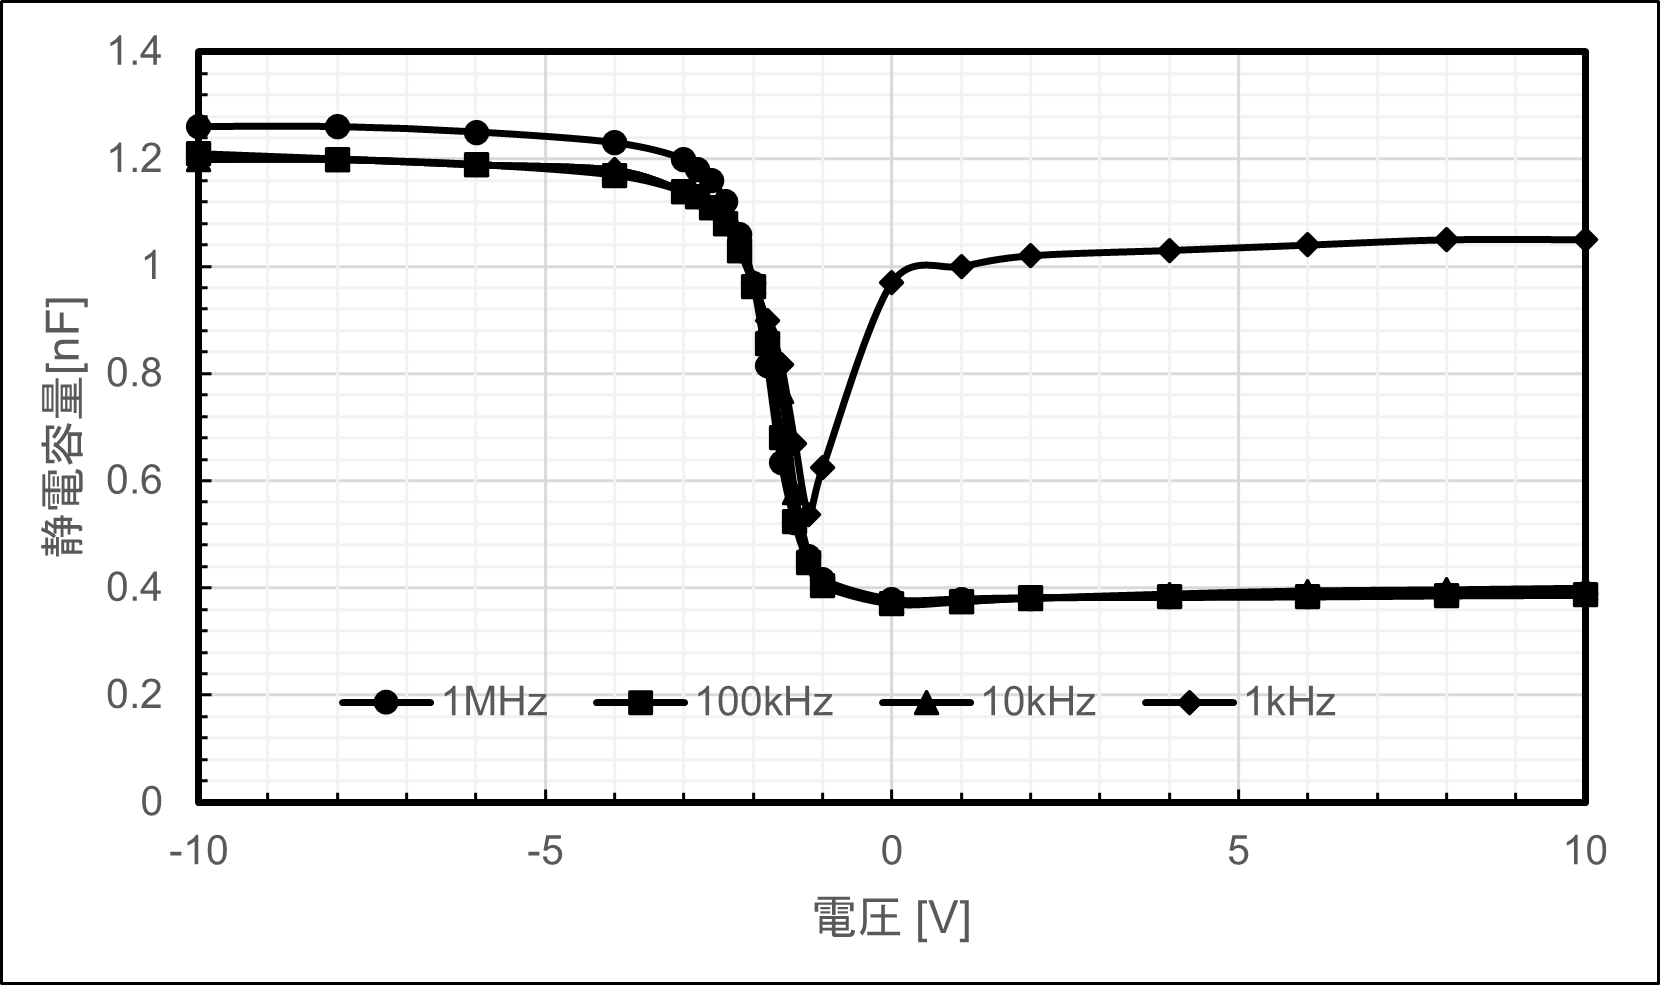
\includegraphics[width = 12cm]{figs/wehacap65.png}
			\caption{酸化時間65分のウェーハの電圧‐静電容量特性のグラフ}
			\label{fig:wehacap65}
			\end{figure}

			\begin{table}[H]
			\begin{center}
			\caption{酸化時間80分のウェーハの電圧‐容量特性}
			\label{tab:wehacap80}
			\begin{tabular}{S|SSSS} \toprule
				&\multicolumn{4}{c}{周波数\,[kHz]ごとの静電容量\,[nF]}\\ \hline
				印加電圧\,[V]&\multicolumn{1}{c}{1000}&\multicolumn{1}{c}{100}&\multicolumn{1}{c}{10}&\multicolumn{1}{c}{1}\\ \hline
				-10 & 1.04 & 0.989 & 0.99 & 0.991 \\
				-8 & 1.04 & 0.985 & 0.988 & 0.989 \\
				-6 & 1.04 & 0.981 & 0.983 & 0.985 \\
				-4 & 1.02 & 0.97 & 0.972 & 0.974 \\
				-3 & 1.01 & 0.952 & 0.955 & 0.956 \\
				-2.8 & 0.999 & 0.947 & 0.948 & 0.949 \\
				-2.6 & 0.989 & 0.938 & 0.939 & 0.94 \\
				-2.4 & 0.975 & 0.924 & 0.925 & 0.926 \\
				-2.2 & 0.953 & 0.904 & 0.905 & 0.906 \\
				-2 & 0.919 & 0.872 & 0.872 & 0.873 \\
				-1.8 & 0.858 & 0.818 & 0.819 & 0.819 \\
				-1.6 & 0.751 & 0.733 & 0.739 & 0.741 \\
				-1.4 & 0.606 & 0.604 & 0.635 & 0.652 \\
				-1.2 & 0.495 & 0.481 & 0.503 & 0.545 \\
				-1 & 0.43 & 0.415 & 0.424 & 0.453 \\
				0 & 0.356 & 0.362 & 0.524 & 0.917 \\
				1 & 0.359 & 0.375 & 0.592 & 0.951 \\
				2 & 0.392 & 0.38 & 0.606 & 0.962 \\
				4 & 0.395 & 0.387 & 0.614 & 0.97 \\
				6 & 0.397 & 0.398 & 0.618 & 0.974 \\
				8 & 0.398 & 0.419 & 0.621 & 0.976 \\
				10 & 0.4 & 0.426 & 0.623 & 0.977 \\ \bottomrule
			\end{tabular}
			\end{center}
			\end{table}

			\begin{figure}[H]
			\centering
			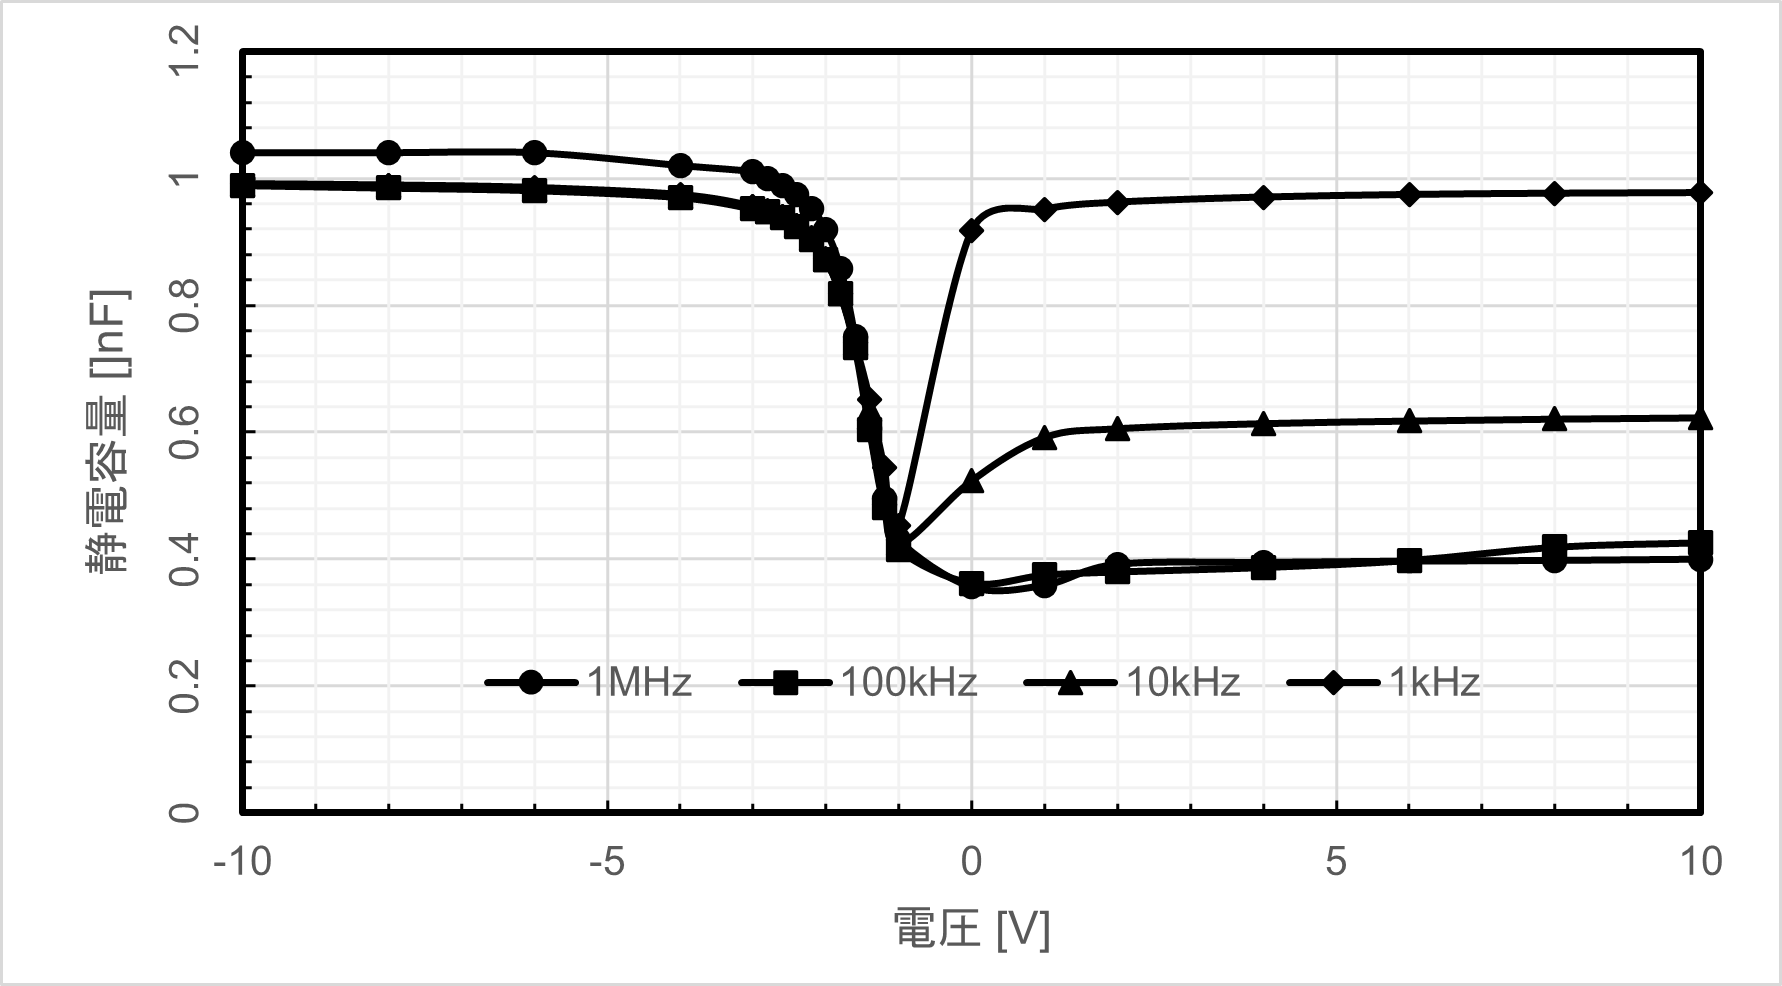
\includegraphics[width = 12cm]{figs/wehacap80.png}
			\caption{酸化時間80分のウェーハの電圧‐静電容量特性のグラフ}
			\label{fig:wehacap80}
			\end{figure}

\section{考察}
\section{所感}
	今回の実験で初めて神戸高専のクリーンルームに入ることができた.
	以前インターンで製薬会社のクリーンルームに入る機会があったが,それと比較するとかなり管理のクラスは低くなっていると実感した.
	クリーンルーム内の装置(特に電気炉)がそこそこ年季が入っているという印象を受けた.
	それ以外では,MOS構造の作成行程でシリコンウェーハの色が酸化時間によって変化するのがとても興味深く,それぞれの手順の時間設定がどのような根拠に基づいて実験を行っているのかが個人的に気にかかる部分であった.
\begin{thebibliography}{99}
\bibitem{ref:指導書}
「実験実習指導書」神戸高専電子工学科 pp,
\end{thebibliography}
\end{document}
